\documentclass[11pt]{article}
\usepackage[a4paper,margin=2cm]{geometry}
\usepackage{setspace}\onehalfspacing
\usepackage[T1]{fontenc}
\usepackage{lmodern}
\usepackage{amsmath,amssymb}
\usepackage{booktabs}
\usepackage{array}
\usepackage{enumitem}
\usepackage{xcolor}
\usepackage{pifont}
\usepackage{tcolorbox}
\usepackage{adjustbox}
\usepackage[hidelinks]{hyperref}
\usepackage{tikz}
\usetikzlibrary{positioning, arrows.meta, fit, calc, backgrounds, shapes.geometric}

% ---- palette (matches the thesis figures) ----
\definecolor{svInk}{HTML}{1A2330}
\definecolor{svBlue}{HTML}{21487A}\definecolor{svBlueT}{HTML}{DBE5F1}
\definecolor{svOrange}{HTML}{E07B2C}\definecolor{svOrangeT}{HTML}{FAE6D2}
\definecolor{svTeal}{HTML}{2C7A7B}\definecolor{svTealT}{HTML}{D6E8E8}
\definecolor{svGreen}{HTML}{4F8A4C}\definecolor{svGreenT}{HTML}{E1EFDD}
\definecolor{svGray}{HTML}{8A9099}\definecolor{svGrayT}{HTML}{ECEEF1}
\definecolor{svRed}{HTML}{C0504D}\definecolor{svRedT}{HTML}{F6DEDD}

\newcommand{\yes}{\textcolor{svGreen}{\ding{51}}}
\newcommand{\no}{\textcolor{svRed}{\ding{55}}}
\newcommand{\shared}{\textcolor{svGreen}{\textbf{shared}}}

\title{\vspace{-1.5cm}\bfseries The Trained Pointer\\[2pt]
\large and how it relates to the Next-POI Engine}
\author{Smart Visit Module --- companion note}
\date{}

% ---- shared tikz node styles ----
\tikzset{
  io/.style   ={draw=svGray,  rounded corners=2pt, fill=svGrayT,   align=center, inner sep=4pt, font=\footnotesize, text=svInk},
  sh/.style   ={draw=svGreen, rounded corners=2pt, fill=svGreenT,  line width=1pt, align=center, inner sep=4pt, font=\footnotesize, text=svInk},
  core/.style ={draw=svBlue,  rounded corners=2pt, fill=svBlueT,   line width=1pt, align=center, inner sep=4pt, font=\footnotesize, text=svInk},
  ptr/.style  ={draw=svOrange,rounded corners=2pt, fill=svOrangeT, line width=1pt, align=center, inner sep=4pt, font=\footnotesize, text=svInk},
  data/.style ={draw=svInk, dashed, rounded corners=2pt, fill=white, align=center, inner sep=4pt, font=\footnotesize, text=svInk},
  arr/.style  ={->, line width=0.8pt, svInk!75},
  darr/.style ={->, line width=0.8pt, svGray, densely dashed},
}

\begin{document}
\maketitle
\vspace{-1.2cm}

\begin{tcolorbox}[colback=svBlueT, colframe=svBlue, arc=2pt, boxrule=0.8pt,
  left=6pt,right=6pt,top=4pt,bottom=4pt]
\textbf{Short answer --- is it similar to your next-POI engine?}
\textbf{Yes, to a large degree.} The Trained Pointer \emph{reuses the very same building blocks}:
the 2-layer GCN over the hybrid POI graph, the learnable user embedding, a GRU of the same size,
and an output distribution over the \emph{whole} POI vocabulary. It is decoded with the
\emph{same} loop-free, reserved-end discipline as Frozen Rollout. It differs in three places:
(1)~the \textbf{output head} (an inner-product \emph{pointer} instead of an MLP),
(2)~what the \textbf{GRU does} (it \emph{decodes the output route} autoregressively from the query,
instead of \emph{encoding the input history}), and
(3)~the \textbf{training signal} (one whole-trajectory example per trip, instead of one example for
every prefix). Point~(3) is why it loses to Frozen Rollout.
\end{tcolorbox}

\section{The two models at a glance}

Both models are built from the \emph{same} encoder stack and only diverge at the ``head'' and in
how they are trained and rolled out. Concretely (file references in \texttt{src/}):

\begin{itemize}[leftmargin=1.4em,itemsep=2pt]
  \item \textbf{Next-POI engine} --- \texttt{src/models/next\_poi.py} (\texttt{NextPOIModel}). Phase~1.
        Predicts the \emph{single next} POI from a session prefix.
  \item \textbf{Trained Pointer} --- \texttt{src/itinerary/pointer\_model.py}
        (\texttt{PointerItineraryModel}). Phase~2, the ``integrated'' alternative.
        Generates a \emph{whole ordered route} from a query.
  \item Both import the \emph{identical} encoder modules \texttt{POIGraphEncoder} and
        \texttt{ContextEncoder} from \texttt{src/models/components.py}. Default dimensions match:
        $d_p=128$ (POI), $d_u=64$ (user), $d_c=32$ (context), $d_h=128$ (GRU).
\end{itemize}

\section{Recap: the Next-POI Engine (Phase 1)}

A 2-layer GCN turns a learnable POI table into graph-aware features
$H=\mathrm{GCN}(\text{graph})\in\mathbb{R}^{|V|\times d_p}$. For each visited POI $p_t$ in the
session, its feature row $H_{p_t}$ is concatenated with a context vector
$c_t=\mathrm{ContextMLP}(\Delta d_t,\Delta t_t)$; a GRU reads the whole prefix and its final state
$h_T$ is combined with the user embedding $e_u$ and scored by an MLP head over all $|V|$ POIs:
\begin{align}
x_t &= [\,H_{p_t}\,\Vert\,c_t\,], &
h_T &= \mathrm{GRU}(x_1,\dots,x_T), \\
z &= [\,h_T\,\Vert\,e_u\,], &
\hat{y} &= \mathrm{MLP}(z)\in\mathbb{R}^{|V|},\quad P(\text{next})=\mathrm{softmax}(\hat{y}).
\end{align}
It is trained with cross-entropy on \emph{every prefix} of every session (a session of length $L$
yields $L-1$ training pairs --- \emph{dense} supervision), early-stopped on validation HR@10.

\section{The Trained Pointer (Phase 2), step by step}

The pointer keeps the GCN encoder $H$ and the user embedding $e_u$, but instead of \emph{reading} a
history it \emph{writes} a route. Figure~\ref{fig:ptr} shows the data flow.

\paragraph{1.\ Encode (shared with Phase~1).}
$H=\mathrm{GCN}(\text{graph})\in\mathbb{R}^{|V|\times d_p}$ and $e_u\in\mathbb{R}^{d_u}$ --- the same
modules and weights-shape as the engine.

\paragraph{2.\ Initialise the decoder from the query.}
The query fixes a start $s$, an end $e$ and a user $u$. These seed the decoder's hidden state:
\begin{equation}
h_0 = \tanh\!\big(W_{\mathrm{init}}\,[\,H_s\,\Vert\,H_e\,\Vert\,e_u\,]\big)\in\mathbb{R}^{d_h}.
\end{equation}
This is something the engine never does --- the engine has no notion of a fixed end.

\paragraph{3.\ Decode the route autoregressively.}
At step $t$ the decoder input is the \emph{previous} POI's GCN feature (plus the
$(\Delta d,\Delta t)$ context in the B-v2 variant), the GRU advances its state, and the state is
projected to a \emph{query vector} $q_t$:
\begin{align}
g_t &= H_{p_{t-1}}\;(\Vert\,c_t\ \text{if context}), &
h_t &= \mathrm{GRU}(g_t,\,h_{t-1}), &
q_t &= W_o\,[\,h_t\,\Vert\,e_u\,]\in\mathbb{R}^{d_p}.
\end{align}

\paragraph{4.\ Point at a POI (the key difference).}
Instead of an MLP head with its own per-POI weights, the score of POI $v$ is just the
\emph{inner product} of the query vector with that POI's GCN feature:
\begin{equation}
\boxed{\ \ell_t(v) = \langle q_t,\,H_v\rangle\ }\qquad \ell_t = q_t H^\top \in\mathbb{R}^{|V|}.
\end{equation}
The output is therefore tied directly to the graph features --- there is no separate classification
matrix to learn.

\paragraph{5.\ Train on whole trajectories; decode loop-free.}
Training is teacher-forced sequence cross-entropy over the \emph{whole} ordered trajectory --- one
example per session (\texttt{ItinerarySeqDataset}), early-stopped on validation pairs-F1. At
inference the route is rolled out with a \textbf{no-revisit mask} (visited POIs set to $-\infty$) and
a \textbf{reserved end} (the last step is forced to $e$), greedy or beam --- exactly the discipline
Frozen Rollout applies to the frozen engine.

\begin{figure}[h]
\centering
\begin{adjustbox}{max width=\textwidth}
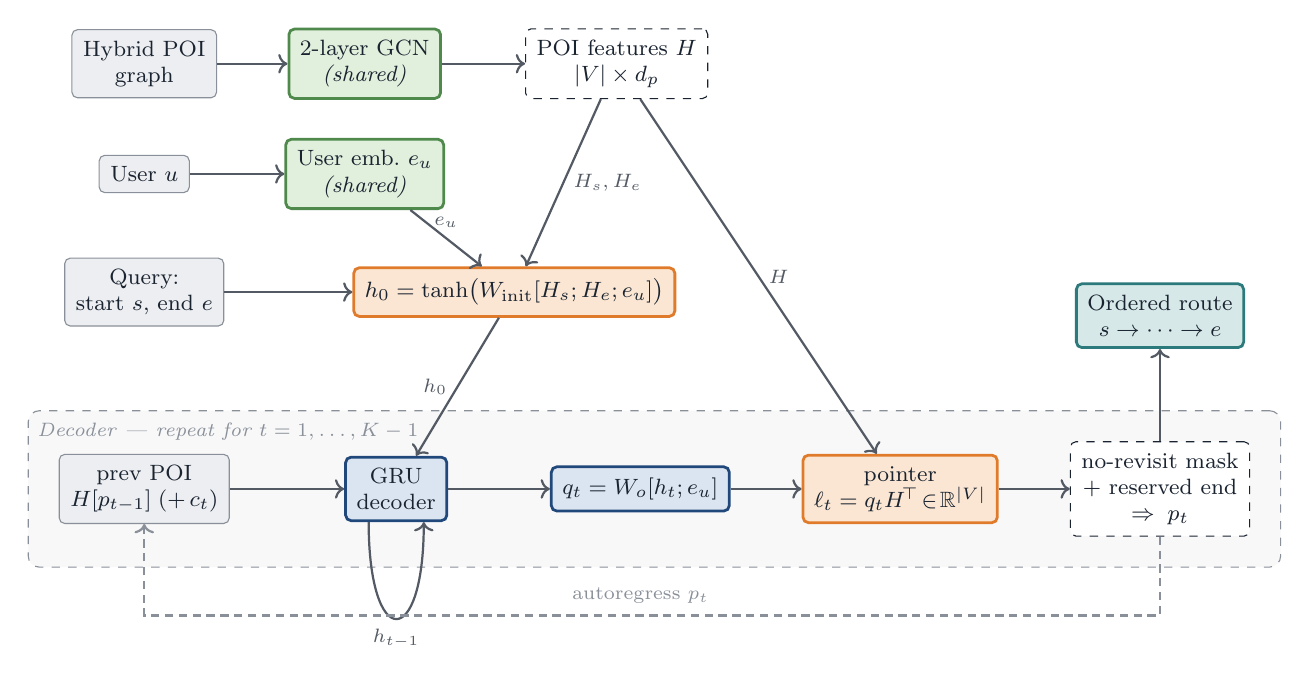
\begin{tikzpicture}[font=\small]
% ---- encode (shared with the engine) ----
\node[io]   (graph) at (0,2.4)   {Hybrid POI\\graph};
\node[sh]   (gcn)   at (2.8,2.4) {2-layer GCN\\\textit{(shared)}};
\node[data] (H)     at (6.0,2.4) {POI features $H$\\$|V|\times d_p$};
\node[io]   (user)  at (0,1.0)   {User $u$};
\node[sh]   (uemb)  at (2.8,1.0) {User emb.\ $e_u$\\\textit{(shared)}};
\node[io]   (query) at (0,-0.5)  {Query:\\start $s$, end $e$};
\node[ptr]  (init)  at (4.7,-0.5){$h_0=\tanh\!\big(W_{\mathrm{init}}[H_s;H_e;e_u]\big)$};

\draw[arr] (graph)--(gcn);
\draw[arr] (gcn)--(H);
\draw[arr] (user)--(uemb);
\draw[arr] (query)--(init);
\draw[arr] (H)    -- node[right,font=\scriptsize]{$H_s,H_e$} (init);
\draw[arr] (uemb) -- node[above,font=\scriptsize]{$e_u$} (init);

% ---- decode row ----
\node[io]   (prev) at (0,-3.0)   {prev POI\\$H[p_{t-1}]\;(+\,c_t)$};
\node[core] (gru)  at (3.2,-3.0) {GRU\\decoder};
\node[core] (op)   at (6.3,-3.0) {$q_t=W_o[h_t;e_u]$};
\node[ptr]  (ptrn) at (9.6,-3.0) {pointer\\$\ell_t=q_t H^{\!\top}\!\in\!\mathbb{R}^{|V|}$};
\node[data] (pick) at (12.9,-3.0){no-revisit mask\\$+$ reserved end\\$\Rightarrow\;p_t$};
\node[draw=svTeal,rounded corners=2pt,fill=svTealT,line width=1pt,align=center,
      inner sep=4pt,font=\footnotesize,text=svInk] (route) at (12.9,-0.8) {Ordered route\\$s\to\cdots\to e$};

\draw[arr] (init) -- node[left,font=\scriptsize]{$h_0$} (gru);
\draw[arr] (prev)--(gru);
\draw[arr] (gru)--(op);
\draw[arr] (op)--(ptrn);
\draw[arr] (ptrn)--(pick);
\draw[arr] (H) -- node[right,font=\scriptsize]{$H$} (ptrn);
\draw[arr] (pick)--(route);
\draw[arr] ([xshift=-3.5mm]gru.south) to[out=-90,in=-90,looseness=6]
       node[below,font=\scriptsize]{$h_{t-1}$} ([xshift=3.5mm]gru.south);
% autoregressive feedback (below the decoder box)
\draw[darr] (pick.south) -- ++(0,-1.0) -| (prev.south);
\node[font=\scriptsize,text=svGray] at (6.3,-4.35) {autoregress $p_t$};

% decoder container
\begin{scope}[on background layer]
\node[draw=svGray,dashed,rounded corners,fill=svGray!6,inner sep=11pt,
      fit=(prev)(gru)(op)(ptrn)(pick),
      label={[font=\scriptsize\itshape,text=svGray,anchor=north west,yshift=-1pt]north west:Decoder --- repeat for $t=1,\dots,K-1$}]{};
\end{scope}
\end{tikzpicture}
\end{adjustbox}
\caption{Architecture of the \textbf{Trained Pointer}. \textcolor{svGreen}{Green} marks the modules
shared with the next-POI engine (the GCN encoder and the user embedding). The query $(s,e,u)$
initialises the GRU \emph{decoder}; at each step the decoder state becomes a query vector $q_t$ whose
\emph{inner product} with every POI feature $H_v$ produces the next-POI scores; the route is rolled
out loop-free with a reserved end. ($e_u$ also enters $q_t$ through $W_o[h_t;e_u]$.)}
\label{fig:ptr}
\end{figure}


\section{Side by side}

Figure~\ref{fig:cmp} lines the two pipelines up; \textcolor{svGreen}{green} marks the modules that are
\shared, \textcolor{svBlue}{blue} the engine-specific head, \textcolor{svOrange}{orange} the
pointer-specific head.

\begin{figure}[h]
\centering
\begin{adjustbox}{max width=\textwidth}
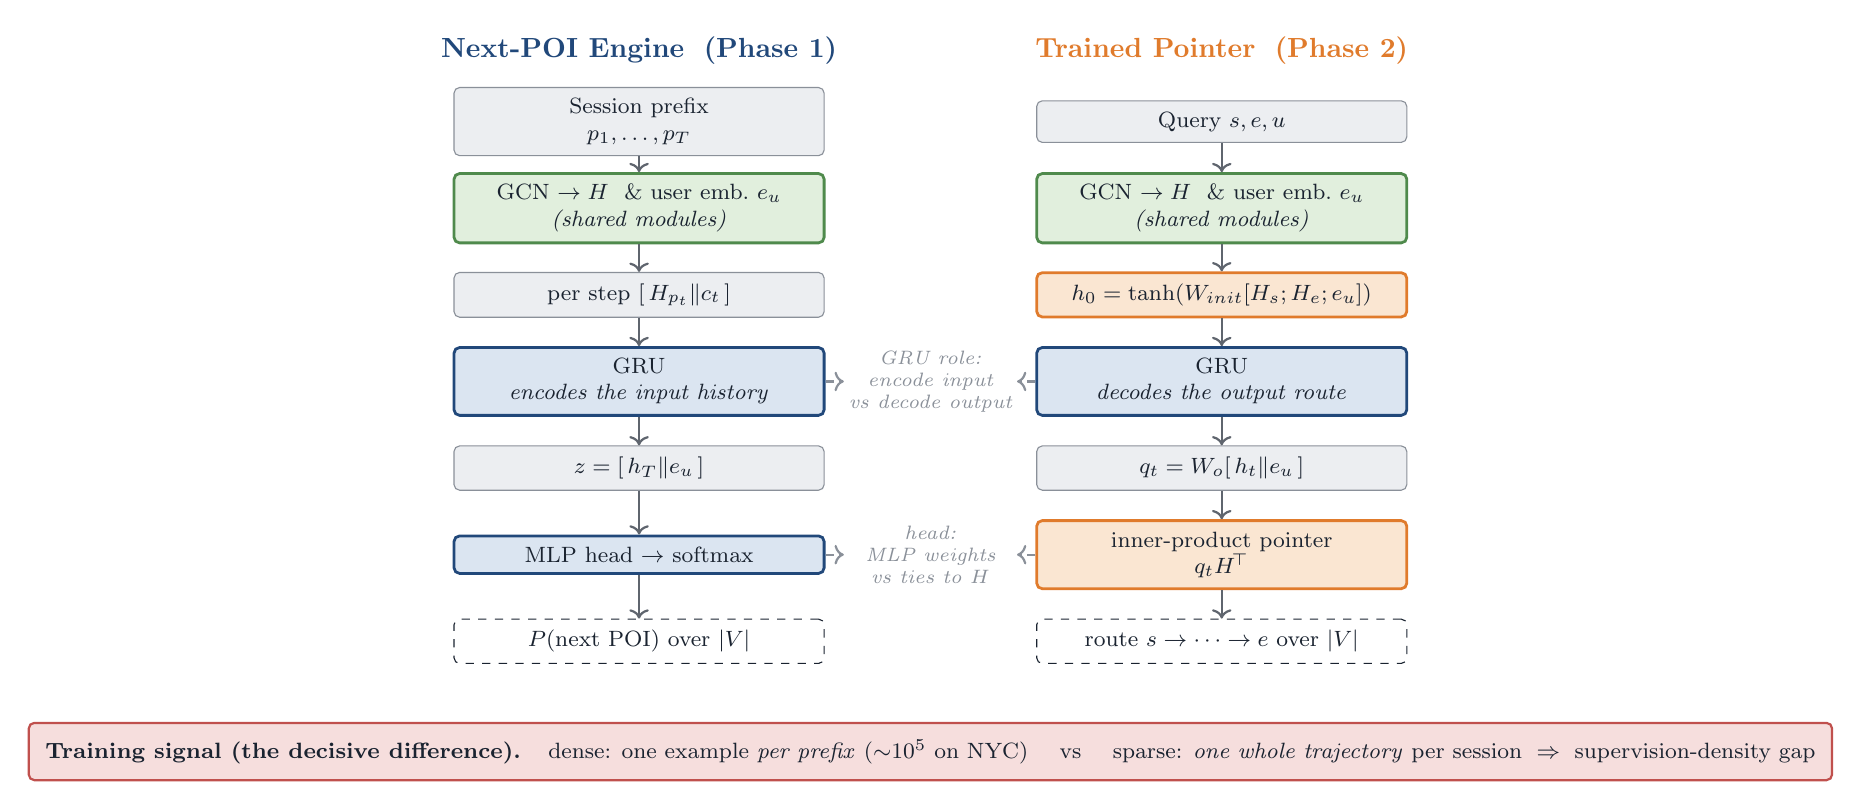
\begin{tikzpicture}[font=\small,
  col/.style={align=center, minimum width=4.7cm, rounded corners=2pt, inner sep=4pt, font=\footnotesize},
  ioc/.style ={col, draw=svGray,  fill=svGrayT,  text=svInk},
  shc/.style ={col, draw=svGreen, fill=svGreenT, line width=1pt, text=svInk},
  coc/.style ={col, draw=svBlue,  fill=svBlueT,  line width=1pt, text=svInk},
  ptc/.style ={col, draw=svOrange,fill=svOrangeT,line width=1pt, text=svInk},
  dac/.style ={col, draw=svInk, dashed, fill=white, text=svInk},
  vlink/.style={->, line width=0.8pt, svInk!70},
  note/.style={align=center, font=\scriptsize\itshape, text=svGray},
]
\def\lx{0}      % left column x
\def\rx{7.4}    % right column x

% titles
\node[font=\bfseries, text=svBlue]   at (\lx,5.0) {Next-POI Engine \;(Phase 1)};
\node[font=\bfseries, text=svOrange] at (\rx,5.0) {Trained Pointer \;(Phase 2)};

% ---- left column (engine) ----
\node[ioc] (e1) at (\lx,4.1) {Session prefix\\$p_1,\dots,p_T$};
\node[shc] (e2) at (\lx,3.0) {GCN $\to H$ \ \&\ user emb.\ $e_u$\\\textit{(shared modules)}};
\node[ioc] (e3) at (\lx,1.9) {per step $[\,H_{p_t}\Vert c_t\,]$};
\node[coc] (e4) at (\lx,0.8) {GRU\\\textit{encodes the input history}};
\node[ioc] (e5) at (\lx,-0.3){$z=[\,h_T\Vert e_u\,]$};
\node[coc] (e6) at (\lx,-1.4){MLP head $\to$ softmax};
\node[dac] (e7) at (\lx,-2.5){$P(\text{next POI})$ over $|V|$};
\foreach \a/\b in {e1/e2,e2/e3,e3/e4,e4/e5,e5/e6,e6/e7}{\draw[vlink] (\a)--(\b);}

% ---- right column (pointer) ----
\node[ioc] (p1) at (\rx,4.1) {Query $s,e,u$};
\node[shc] (p2) at (\rx,3.0) {GCN $\to H$ \ \&\ user emb.\ $e_u$\\\textit{(shared modules)}};
\node[ptc] (p3) at (\rx,1.9) {$h_0=\tanh(W_{init}[H_s;H_e;e_u])$};
\node[coc] (p4) at (\rx,0.8) {GRU\\\textit{decodes the output route}};
\node[ioc] (p5) at (\rx,-0.3){$q_t=W_o[\,h_t\Vert e_u\,]$};
\node[ptc] (p6) at (\rx,-1.4){inner-product pointer\\$q_t H^{\!\top}$};
\node[dac] (p7) at (\rx,-2.5){route $s\to\cdots\to e$ over $|V|$};
\foreach \a/\b in {p1/p2,p2/p3,p3/p4,p4/p5,p5/p6,p6/p7}{\draw[vlink] (\a)--(\b);}

% ---- contrast annotations in the gap ----
\node[note] at (3.7,0.8)  {GRU role:\\encode input\\vs decode output};
\node[note] at (3.7,-1.4) {head:\\MLP weights\\vs ties to $H$};
\draw[darr] (e4.east)--(2.6,0.8); \draw[darr] (p4.west)--(4.8,0.8);
\draw[darr] (e6.east)--(2.6,-1.4); \draw[darr] (p6.west)--(4.8,-1.4);

% ---- bottom banner: the key difference ----
\node[draw=svRed, fill=svRedT, rounded corners=2pt, line width=0.8pt, align=center,
      font=\footnotesize, text=svInk, minimum width=12cm, inner sep=6pt] at (3.7,-3.9)
   {\textbf{Training signal (the decisive difference).} \;
    dense: one example \emph{per prefix} ($\sim$$10^5$ on NYC) \quad vs \quad
    sparse: \emph{one whole trajectory} per session \;$\Rightarrow$\; supervision-density gap};
\end{tikzpicture}
\end{adjustbox}
\caption{The next-POI engine and the Trained Pointer side by side.
\textcolor{svGreen}{Green} = modules shared by both (GCN encoder $+$ user embedding);
\textcolor{svBlue}{blue} = the engine's MLP head; \textcolor{svOrange}{orange} = the pointer-specific
parts (query-initialised decoder and inner-product head). Same encoder, different head, and --- the
decisive difference --- a far sparser training signal.}
\label{fig:cmp}
\end{figure}


\begin{table}[h]
\centering\small
\renewcommand{\arraystretch}{1.25}
\begin{tabular}{>{\raggedright\arraybackslash}p{3.5cm} >{\raggedright\arraybackslash}p{5.0cm} >{\raggedright\arraybackslash}p{5.0cm}}
\toprule
& \textbf{Next-POI engine} & \textbf{Trained Pointer} \\
\midrule
GCN graph encoder      & \yes\ \texttt{POIGraphEncoder} & \yes\ \emph{same} \texttt{POIGraphEncoder} \\
User embedding $e_u$   & \yes\ $d_u=64$ & \yes\ \emph{same} ($d_u=64$) \\
$(\Delta d,\Delta t)$ context & \yes\ always & \yes\ optional (B-v2 only) \\
GRU                    & encodes the \emph{input} history & decodes the \emph{output} route (autoregressive) \\
Hidden init            & zeros (reads a prefix) & $h_0=\tanh(W_{init}[H_s;H_e;e_u])$ from the query \\
Output head            & \textcolor{svBlue}{MLP $\to$ softmax over $|V|$} & \textcolor{svOrange}{inner product $q_t H^\top$} \\
End POI                & not modelled & given; reserved at the last step \\
Training examples      & every prefix ($L\!-\!1$ per session; $\sim$$10^5$ on NYC) & one whole trajectory per session \\
Early-stop metric      & validation HR@10 & validation pairs-F1 \\
Output                 & a ranked next POI & an ordered, loop-free route $s\!\to\!\cdots\!\to\!e$ \\
\bottomrule
\end{tabular}
\caption{What is shared (\yes) and what differs between the two models.}
\label{tab:cmp}
\end{table}

\section{Why the Pointer does \emph{not} beat Frozen Rollout}

On Foursquare NYC (length-$\ge\!3$ test, $n=2{,}880$), decoding the \emph{frozen} engine
(\textbf{Frozen Rollout}) actually \emph{beats} the purpose-trained pointer:

\begin{center}\small
\begin{tabular}{lcc}
\toprule
Method & Type & pairs-F1 \\
\midrule
\textbf{Frozen Rollout} (greedy) & decoupled & \textbf{0.289} \\
Frozen Rollout (beam~3) & decoupled & 0.290 \\
Trained Pointer v1 (no context) & integrated & 0.259 \\
Trained Pointer v2 ($+$ context) & integrated & 0.261 \\
\bottomrule
\end{tabular}
\end{center}

\noindent The decisive reason is \textbf{supervision density}. The engine learns from every prefix of
every session ($\sim$$10^5$ next-POI examples on NYC); the pointer sees only \emph{one}
whole-trajectory example per session --- far fewer gradient signals, and it trains its encoder from
scratch rather than reusing a converged one. Two secondary effects: the v1 pointer conditions only on
the previous POI's feature (adding $(\Delta d,\Delta t)$ in v2 recovers a little), and beam search
barely helps either model ($+0.0015$), showing the limit is the \emph{scorer}, not the search. The
honest lesson: \emph{naively training a dedicated itinerary model does not automatically beat
cleverly decoding a strong next-POI model.}

\begin{tcolorbox}[colback=svGrayT, colframe=svGray, arc=2pt, boxrule=0.6pt,
  left=6pt,right=6pt,top=4pt,bottom=4pt]
\textbf{In one line.} The Trained Pointer is your next-POI engine's encoder (GCN $+$ user embedding)
re-wired into a query-initialised, autoregressive route \emph{decoder} with an inner-product head ---
same parts, different head, sparser training --- and that sparser training is exactly why the simple
decoupled Frozen Rollout wins. A lighter sibling of this pointer is used for the Flickr literature
benchmark (\texttt{src/flickr/pointer.py}).
\end{tcolorbox}

\end{document}
